
\documentclass[10pt,a4paper]{article}
\usepackage[T1]{fontenc}
\usepackage{tikz}
\usepackage[margin=1cm]{geometry}
\begin{document}
\section*{Introduction}
The Red-Black tree is a self-balancing binary search tree where each node is either red or black. The tree maintains balance through several properties that ensure it remains approximately balanced.

\subsection*{Step-by-Step Process}
The following figures illustrate the Red-Black tree at various stages of the deletion and balancing process:


\begin{figure}[h!]
\centering

\begin{minipage}{0.8\textwidth}
    \centering
    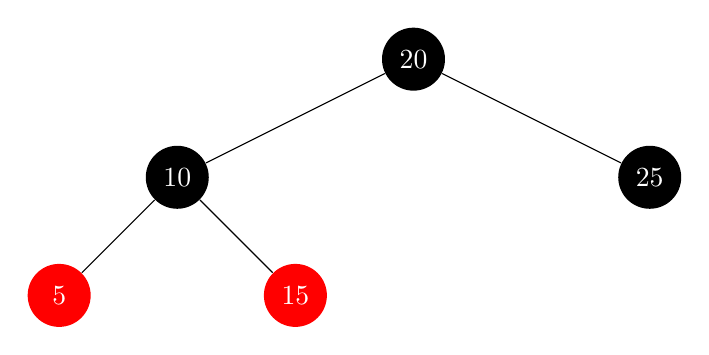
\begin{tikzpicture}[level distance=15mm, sibling distance=20mm]
        \tikzstyle{every node}=[circle,inner sep=1pt, minimum size=8mm]
        \tikzstyle{level 1}=[sibling distance=60mm]
        \tikzstyle{level 2}=[sibling distance=30mm]
        \tikzstyle{level 3}=[sibling distance=15mm]
        \tikzstyle{level 4}=[sibling distance=10mm]
        \node [fill=black, text=white] {20} child {node [fill=black, text=white] {10} child {node [fill=red, text=white] {5} } child {node [fill=red, text=white] {15} }} child {node [fill=black, text=white] {25} };
    \end{tikzpicture}
    \caption{Initial Tree}
\end{minipage}
\vspace{1cm}

\begin{minipage}{0.8\textwidth}
    \centering
    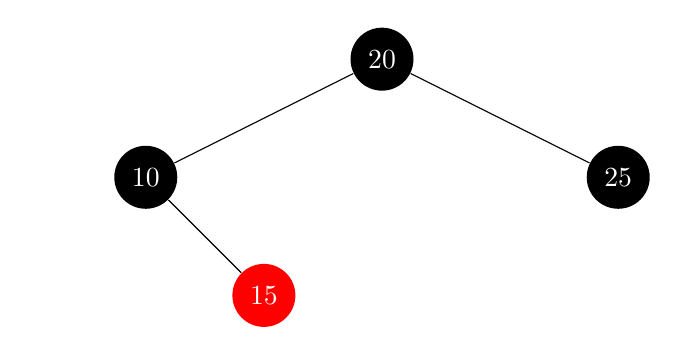
\begin{tikzpicture}[level distance=15mm, sibling distance=20mm]
        \tikzstyle{every node}=[circle,inner sep=1pt, minimum size=8mm]
        \tikzstyle{level 1}=[sibling distance=60mm]
        \tikzstyle{level 2}=[sibling distance=30mm]
        \tikzstyle{level 3}=[sibling distance=15mm]
        \tikzstyle{level 4}=[sibling distance=10mm]
        \node [fill=black, text=white] {20} child {node [fill=black, text=white] {10} child[fill=none] {edge from parent[draw=none]} child {node [fill=red, text=white] {15} }} child {node [fill=black, text=white] {25} };
    \end{tikzpicture}
    \caption{Step 2}
\end{minipage}
\vspace{1cm}

\begin{minipage}{0.8\textwidth}
    \centering
    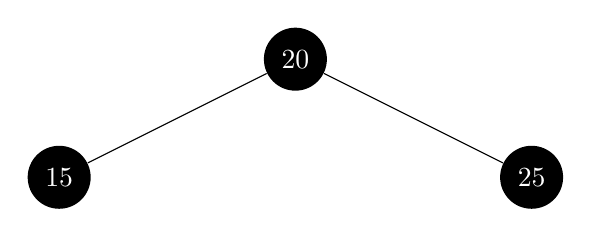
\begin{tikzpicture}[level distance=15mm, sibling distance=20mm]
        \tikzstyle{every node}=[circle,inner sep=1pt, minimum size=8mm]
        \tikzstyle{level 1}=[sibling distance=60mm]
        \tikzstyle{level 2}=[sibling distance=30mm]
        \tikzstyle{level 3}=[sibling distance=15mm]
        \tikzstyle{level 4}=[sibling distance=10mm]
        \node [fill=black, text=white] {20} child {node [fill=black, text=white] {15} } child {node [fill=black, text=white] {25} };
    \end{tikzpicture}
    \caption{Step 3}
\end{minipage}
\vspace{1cm}

\end{figure}
\newpage

\end{document}
